\documentclass[9pt]{beamer}
\usetheme[progressbar=frametitle]{metropolis}
\usepackage{appendixnumberbeamer}
\usepackage{braket}
\usepackage{booktabs}
\usepackage[scale=2]{ccicons}
\usepackage{amsmath}
\usepackage{amssymb}
\usepackage{pgfplots}
\usepackage{tikz}
\usepackage{physics}
\usepgfplotslibrary{dateplot}
\usepackage{xspace}
\newcommand{\themename}{\textbf{\textsc{metropolis}}\xspace}
\usepackage{graphicx}


\title{Physics-informed neural networks (PINN) with \\a mathematically informed architecture \\for solving the nuclear decay equation}
\date{}
\author{Miha Pompe\\Supervised by: Dr. A. Adelmann, A. Alb\`a, Dr. R. Boiger}
\titlegraphic{
\includegraphics[width=2cm]{download_2.png}\hspace*{6cm}~%
   
\includegraphics[width=2cm]{PSI-Logo_narrow_30k.jpg}
}

\begin{document}
\maketitle

\begin{frame}[fragile]{Outline}
\begin{itemize}
    \item Nuclear decay equation
    \item Physics-informed neural networks
    \item Implementation
    \item Results
    \item Conclusion
\end{itemize}
\end{frame}


\begin{frame}[fragile]{Nuclear decay equation}
\begin{itemize}
    \item We are interested in the time evolution of isotope concentrations in spent nuclear fuel and in nuclear cores.
    \item The decay equation:
    \begin{equation*}\label{eq:decay_eq}
        \frac{d\mathbf{N}(t)}{dt} = A \mathbf{N}(t) \,,\qquad \text{with} \quad \mathbf{N}(t=0) = \mathbf{N}_0 \,.
    \end{equation*}
    \item $A \in \mathbb{R}^{n \times n}$ can be very large ($n = 4000$) and stiff $|A| = \frac{|\lambda_{max}|}{|\lambda_{min}|} > 10^{20}$.
    \item Formal solution of the equation is $\mathbf{N}(t) = e^{At}\mathbf{N}(0)$\footnotemark.
    \item CRAM and Pad\'e are rational approximation methods that estimate the exponential function\footnotemark.
    \begin{itemize}
        \item CRAM: accurate, less reliable for burnup matrices.
        \item Pad\'e: fast, but inaccurate in stiff cases.
        \item Runge-Kutta: accurate, but slow. 
    \end{itemize}
\end{itemize}
\footnotetext[1]{Centar (2013)}
\footnotetext[2]{Pusa (2010)}
\end{frame}


\begin{frame}[fragile]{Nuclear decay equation}
\begin{columns}[M] % Top alignment of columns
\begin{column}{0.45\textwidth} % Left column
\begin{itemize}
    \item A matrix can be a burnup or decay matrix.
    \item A general solution can be written in form of $^2$:
    \begin{align*}\label{eq:complex_sol}
    \mathbf{N}(t) = \sum_{i=1}^n \mathbf{a}_i\cos(\Im(\lambda_i)t)e^{\Re(\lambda_i)t}\\
    +\mathbf{b}_i\sin(\Im(\lambda_i)t)e^{\Re(\lambda_i)t}.
    \end{align*}
    \item Solution for the decay problem $^2$:
    \begin{equation*}\label{eq:real_sol}
    \mathbf{N}(t) = \sum_{i=1}^n \mathbf{a}_i e^{\lambda_i t}.
    \end{equation*}
\end{itemize}
\end{column}
\begin{column}{0.55\textwidth} % Right column
\begin{figure}
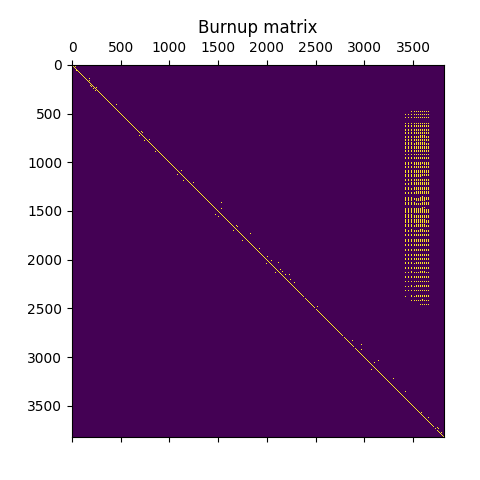
\includegraphics[width=\textwidth]{burnup_matrix.png}
% \caption{Caption of the photo}
\end{figure}
\end{column}
\end{columns}
\footnotetext[2]{Pusa (2010)}
\end{frame}


\begin{frame}[fragile]{Physics-informed neural networks (PINN)}
\begin{itemize}
    \item PINNs are comprised of two parts, neural network and physics-based loss function. They are used to solve PDEs.\footnotemark
    \begin{figure}
        \centering
        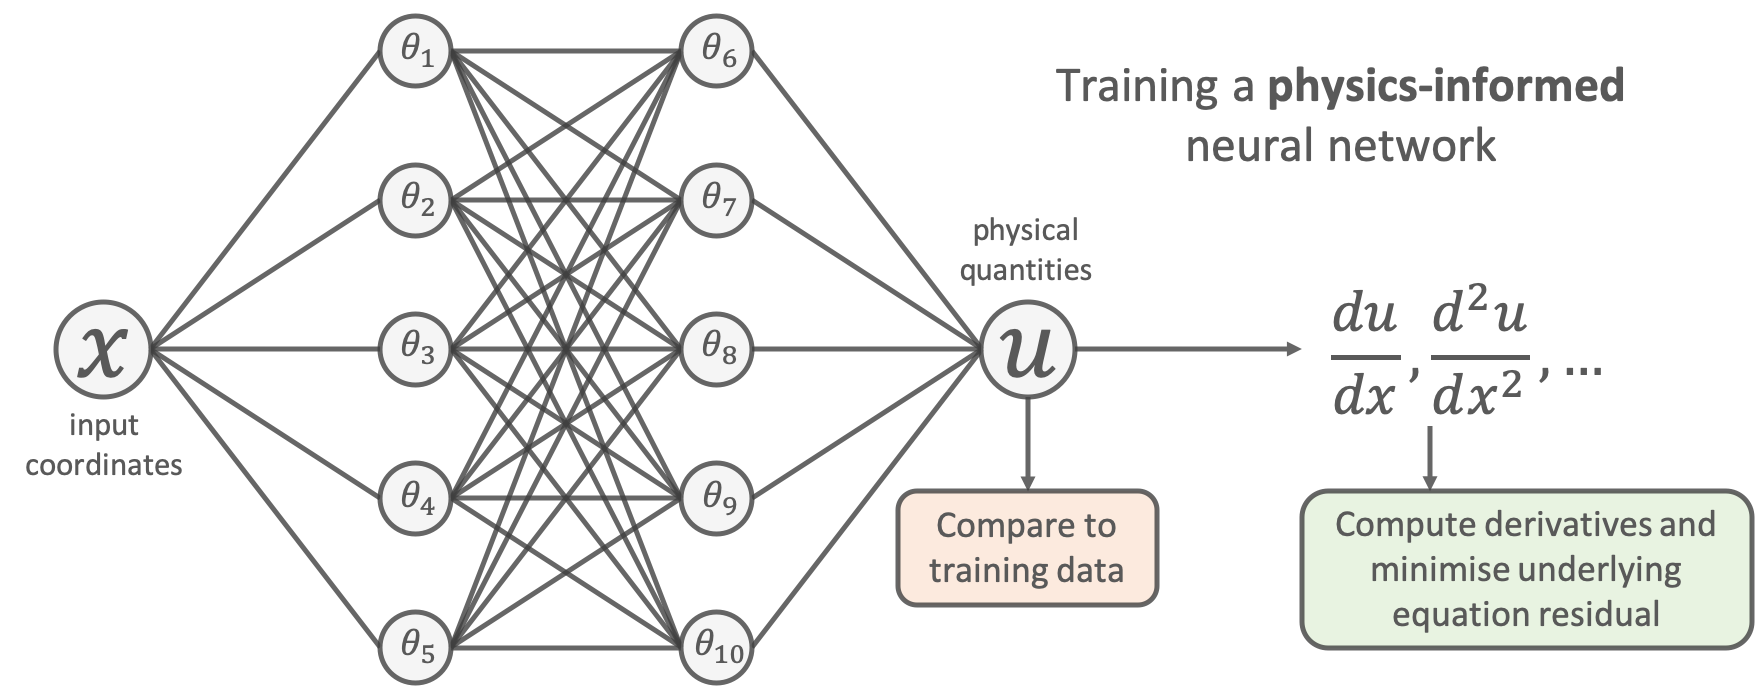
\includegraphics[width = 7.0 cm]{pinn.png}
        % \caption{Caption}
        % \label{fig:my_label}
    \end{figure}
    \item Physics-based loss function:
    \begin{align*}
        \mathcal{L}_{ODE} = \left|\frac{d\mathbf{N}(t)}{dt} - A \mathbf{N}(t)\right|^2, \quad
        \mathcal{L}_{IC} = \left|\mathbf{N}(0) - \mathbf{N}_0\right|^2
    \end{align*}
    \item The weights of the network are adjusted to minimize both the prediction error and the physics-based loss.
    \item Potential use case of PINNs is much faster uncertainty analysis compared to other methods.
\end{itemize}
\footnotetext[3]{Raissi (2019)}
\end{frame}


\begin{frame}[fragile]{Implementation - Decay problem}
\begin{columns}[M] % Top alignment of columns
\begin{column}{0.45\textwidth} % Left column
\begin{itemize}
\item Solution for decay problem is in form $\mathbf{N}(t) = \sum_{i=0}^n \mathbf{a}_i e^{\lambda_i t} $\\$\Leftrightarrow  \mathbf{N}(t) = M\mathbf{h},\text{ with }$\\$ \mathbf{h}=(e^{\lambda_1 t}, ..., e^{\lambda_n t}).$
\item Input and output layer with one hidden layer.
\item Change the activation function to $\sigma(z) = e^z$.
\item Constraining the weights of the network: fix weights in input layer, M triangular.
\item Trainable weights $\frac{n(n+1)}{2}$.
\item Reduction in number of trainable weights and hyperparameters.
\end{itemize}
\end{column}
\begin{column}{0.55\textwidth} % Right column
\begin{figure}
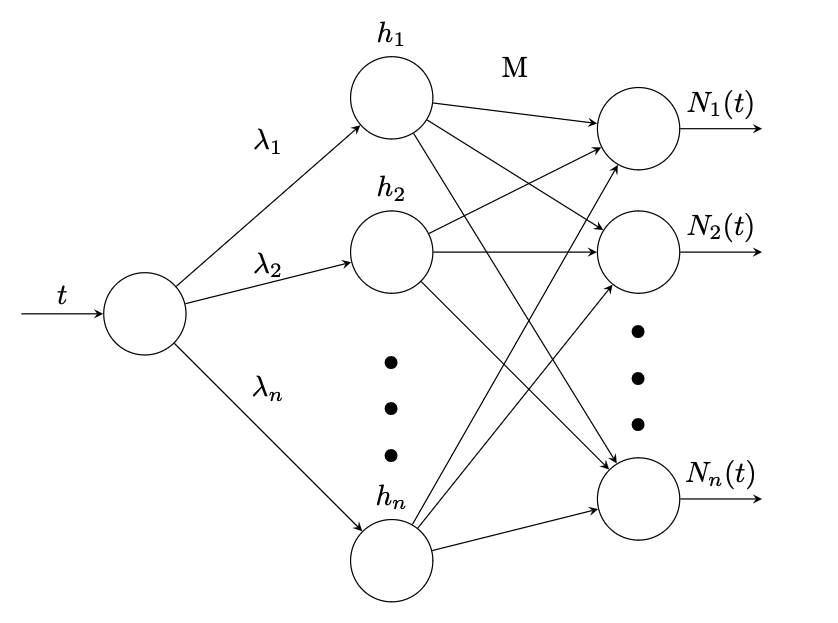
\includegraphics[width=\textwidth]{Screenshot 2023-05-21 at 14.27.59.png}
% \caption{Caption of the photo}
\end{figure}
\end{column}
\end{columns}
\end{frame}


\begin{frame}[fragile]{Implementation - Burnup problem}
\begin{columns}[M] % Top alignment of columns
\begin{column}{0.55\textwidth} % Right column
\begin{figure}
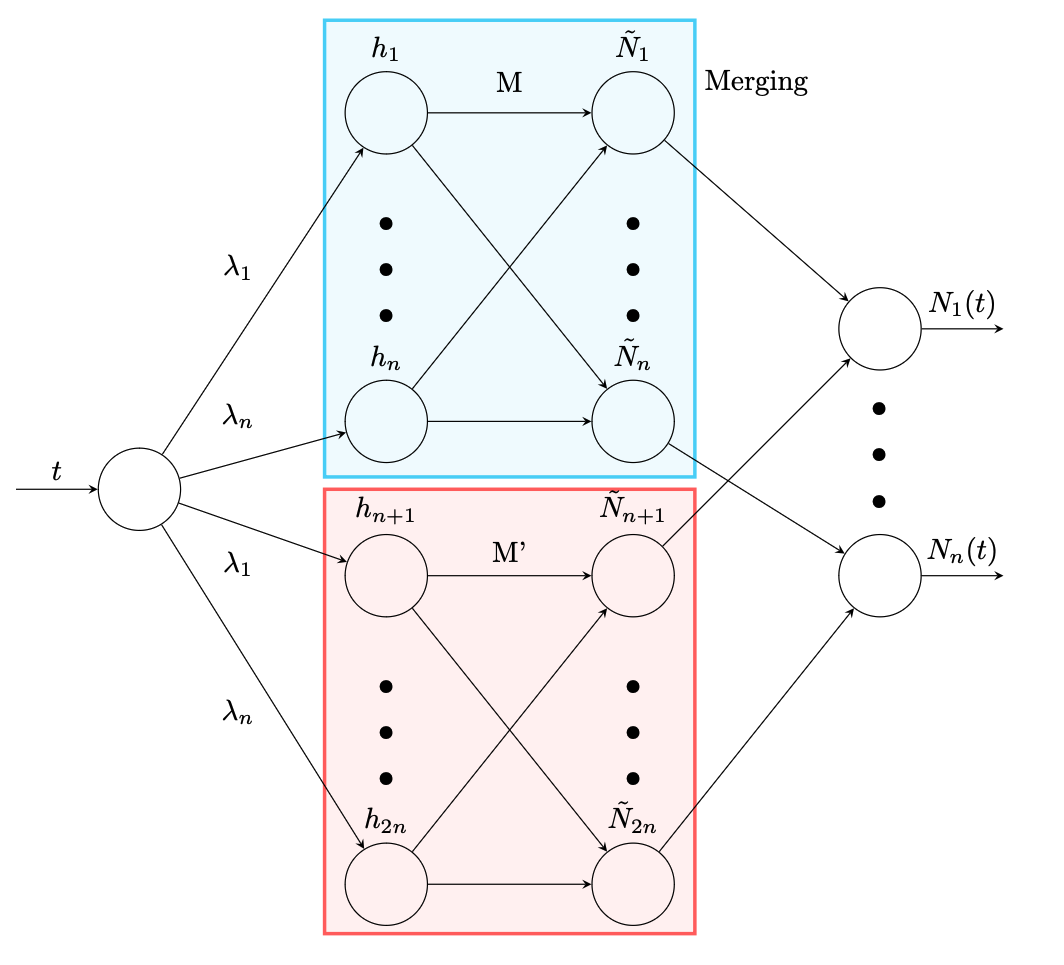
\includegraphics[width=\textwidth]{Screenshot 2023-05-21 at 14.28.14.png}
% \caption{Caption of the photo}
\end{figure}
\end{column}
\begin{column}{0.45\textwidth} % Left column
\begin{itemize}
\item Solution of the burnup problem is $N_j(t) = M_{ij} h_i + M'_{ij} h_{n+i}$, where $h_i = \cos(\Im(\lambda_i) t) e^{\Re(\lambda_i) t},$ $h_{n+i} = \sin(\Im(\lambda_i) t) e^{\Re(\lambda_i) t}$.
\item Two neural networks and a merging layer.
\item Two activation functions.
\item Fix weights in input layer.
\item Trainable weights $2n^2$.
\end{itemize}
\end{column}
\end{columns}
\end{frame}


\begin{frame}[fragile]{Results - Solution}
\begin{itemize}
\item Analysis done on a decay matrix with initial conditions $N_i(0) = 1$ for all $i$.
\item The method also achieves similar performance with burnup matrices.
\begin{figure}
    \centering
    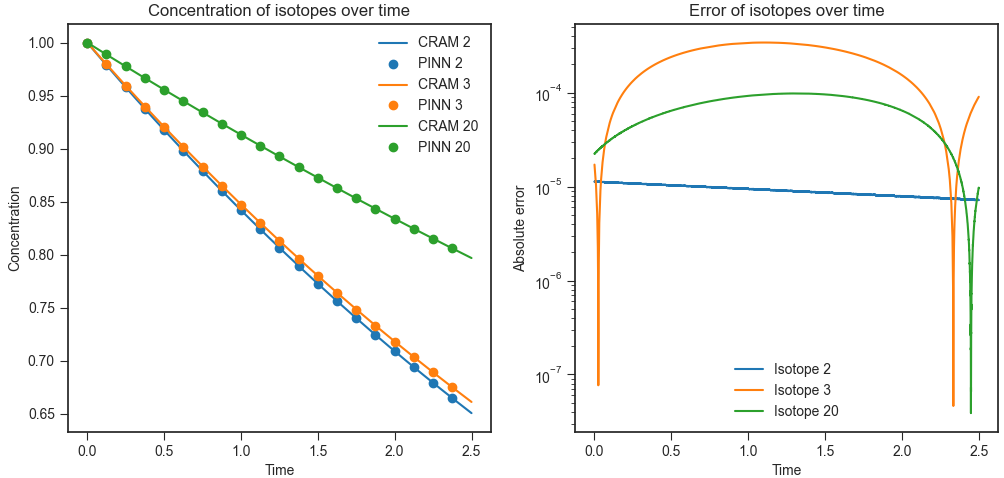
\includegraphics[width=0.9\textwidth]{decay_over_time_trimed.png}
    % \caption{Caption}
    \label{fig:my_label}
\end{figure}
\item Decay matrix of size 50$\times$50, with stiffness $10^{16}$ (default test case).
\item Final error defined as the sum of absolute errors for each isotope at final time, $\Delta N(t_{max}) &= \left|\mathbf{N}_{CRAM}(t_{max}) - \mathbf{N}(t_{max})\right|$.
\end{itemize}
\end{frame}


\begin{frame}[fragile]{Results - Weight ratio}
The total loss is a weighted sum of both losses:
\begin{equation*}
    \mathcal{L} = \frac{w_{ODE} \mathcal{L}_{ODE} + w_{IC} \mathcal{L}_{IC}}{w_{ODE} + w_{IC}}.
\end{equation*}
Define weight ratio as $w = w_{IC}/w_{ODE}$. It turns out that it is a very important hyperparameter that should be tuned for each test case.
\begin{figure}
    \centering
    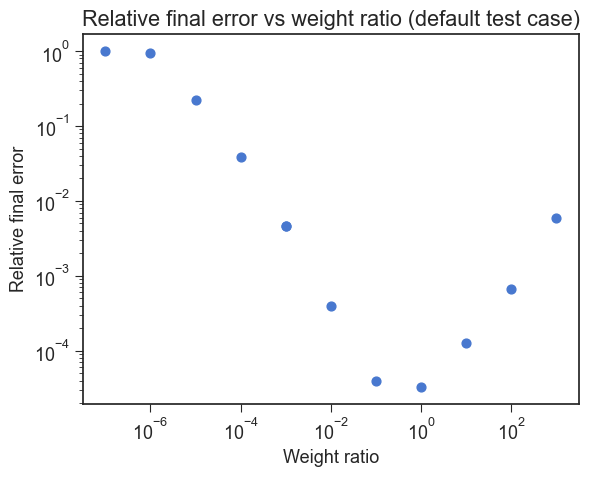
\includegraphics[width= 5.5cm]{error_vs_ratio.png}
    % \caption{Caption}
    \label{fig:my_label}
\end{figure}
\end{frame}


\begin{frame}[fragile]{Results - Dependence on stiffness}
\begin{itemize}
    \item Final relative error slightly rises up to a stiffness cutoff at round $10^{19}$.
    \item Computation time for PINN is roughly constant up to the stiffness cutoff. Computation time for CRAM is independent of stiffness.
    \item All the simulations were done on CPU, but code also runs on GPU, where the computation time is lower.
\end{itemize}
\begin{figure}
    \centering
    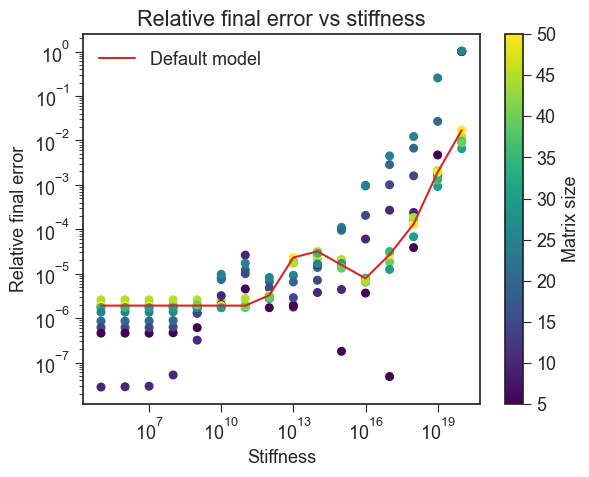
\includegraphics[width=0.49\textwidth]{error_vs_stiffness_multi.png}
    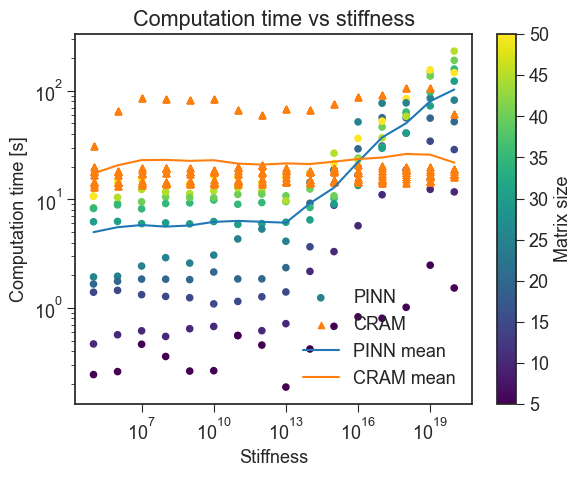
\includegraphics[width=0.49\textwidth]{time_vs_stiffness_multi.png}
    % \caption{Caption}
    \label{fig:my_label}
\end{figure}
\end{frame}


\begin{frame}[fragile]{Results - Dependence on matrix size}
\begin{itemize}
    \item The relative final error slightly dependent on matrix size.
    \item Computation time scales linearly with the size of the matrix, as does the CRAM method for $n > 45$.
    \item All matrices derived from ENDF/B VII.1 nuclear data library.
\end{itemize}
\begin{figure}
    \centering
    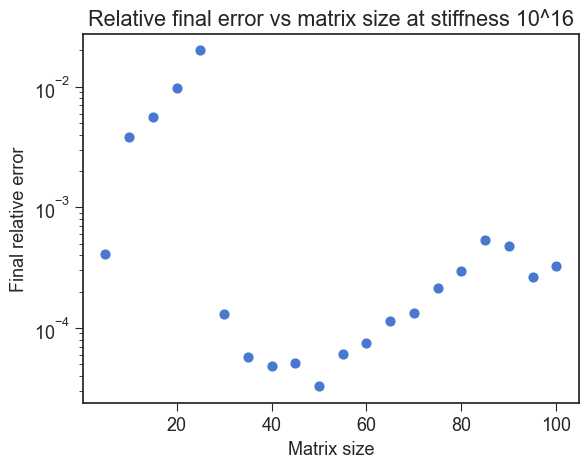
\includegraphics[width=0.49\textwidth]{error_vs_size.png}
    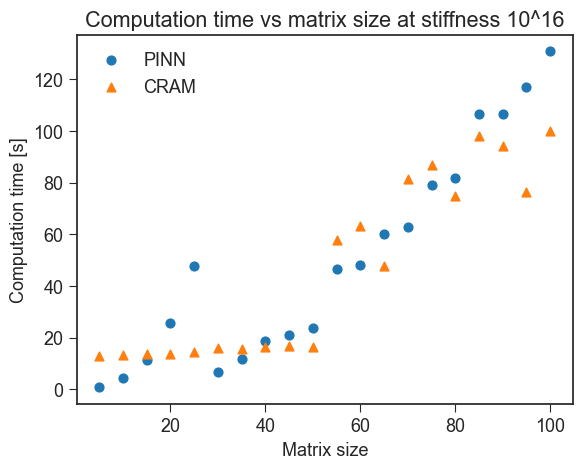
\includegraphics[width=0.49\textwidth]{time_vs_size.png}
    % \caption{Caption}
    \label{fig:my_label}
\end{figure}
\end{frame}


\begin{frame}[fragile]{Conclusions}
The method works:
\begin{itemize}
\item for both decay and burnup matrices,
\item for any matrix size (tested on up to 442$\times$442 burnup matrix, limited by memory and time),
\item for any stiffness up to about $|A| = 10^{19}$,
\item faster than CRAM for matrices with stiffness under $10^{16}$, with relative final error of around $10^{-5}$,
\item faster and can handle bigger and more stiff problem than general purpose PINNs.
\end{itemize}
Future work:
\begin{itemize}
    \item improve the performance at bigger stiffnesses,
    \item find an optimal way of setting the weight ratio.
\end{itemize}
\end{frame}


\begin{frame}[fragile]{References}
\footnotesize\begin{enumerate}
    \item J. Cetnar \textit{General solution of Bateman equations for nuclear transmutations.} Annals of Nuclear Energy (2013) https://www.sciencedirect.com/science/article/pii/\\S0306454906000284#:~:text=The\%20Bateman\%20equations\%20for\%20radioactive,\\decay\%20constant\%20of\%20ith\%20nuclide
    \item M. Pusa and J. Leppänen. \textit{Computing the Matrix Exponential in Burnup Calculations.} Nuclear Science and Engineering: 164, 140–150, (2010) https://www.tandfonline.com/doi/abs/10.13182/NSE09-14
    \item M. Raissi, P. Perdikaris, and G. E. Karniadakis.
         \textit{Physics-informed neural networks: A deep learning framework for solving forward and inverse problems involving nonlinear partial differential equations.}
         Journal of Computational Physics, 378:686–707, (2019) https://www.sciencedirect.com/science/article/pii/S0021999118307125
    \item H. Baty. \textit{Solving stiff ordinary differential equations using physics informed neural networks (PINNs): simple recipes to improve training of vanilla-PINNs.} (2023)
    \item G. Pacifico and A. Adelmann, \textit{Solving the Decay Equation using a Physics Informed Neural Network (PINN).} (2023)
\end{enumerate}
\end{frame}


\begin{frame}[fragile]{Backup slides - More data on stiffness dependence}
\begin{figure}
    \centering
    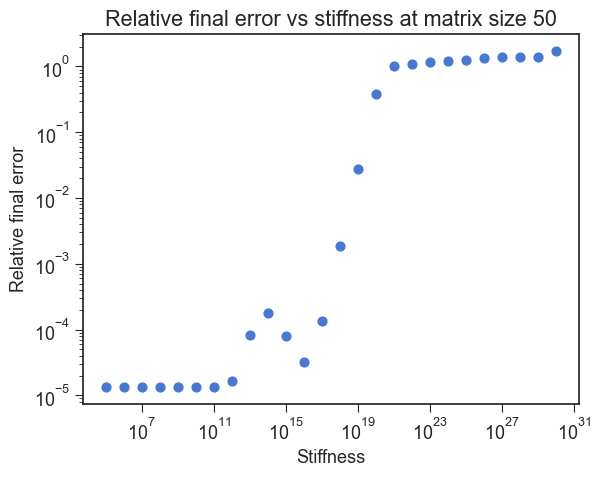
\includegraphics[width=0.49\textwidth]{error_vs_stiffness.png}
    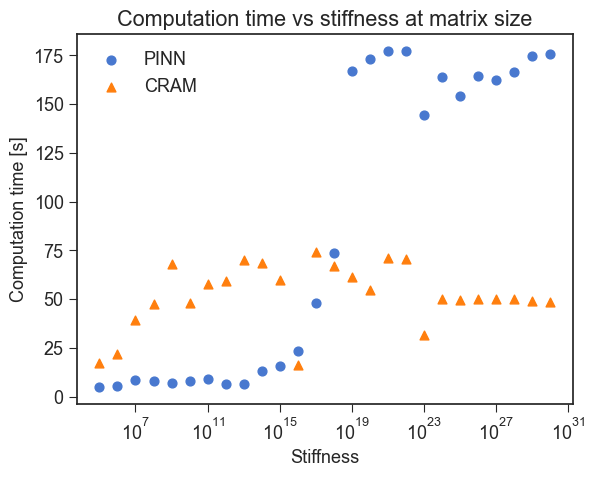
\includegraphics[width=0.49\textwidth]{time_vs_stiffness.png}
    % \caption{Caption}
    \label{fig:my_label}
\end{figure}
\end{frame}


\begin{frame}[fragile]{Backup slides - More data on size dependence}
\begin{figure}
    \centering
    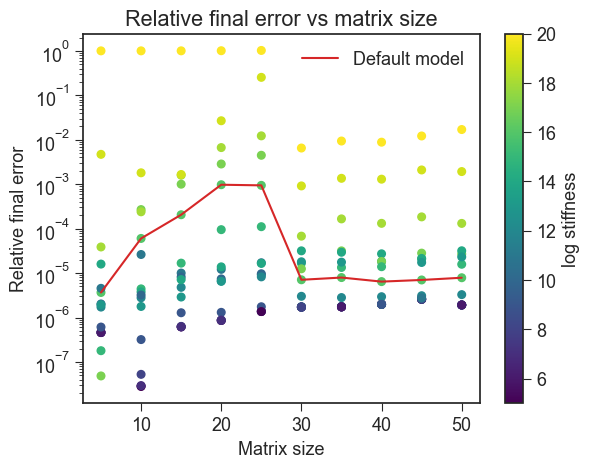
\includegraphics[width=0.49\textwidth]{error_vs_size_multi.png}
    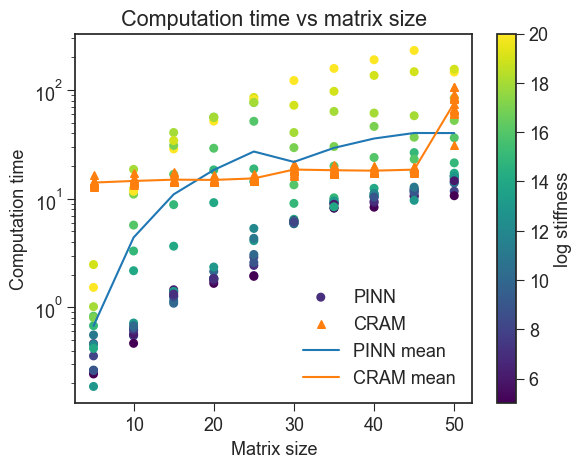
\includegraphics[width=0.49\textwidth]{time_vs_size_multi.png}
    % \caption{Caption}
    \label{fig:my_label}
\end{figure}
\end{frame}


\begin{frame}[fragile]{Backup slides - Burnup problem}
\begin{figure}
    \centering
    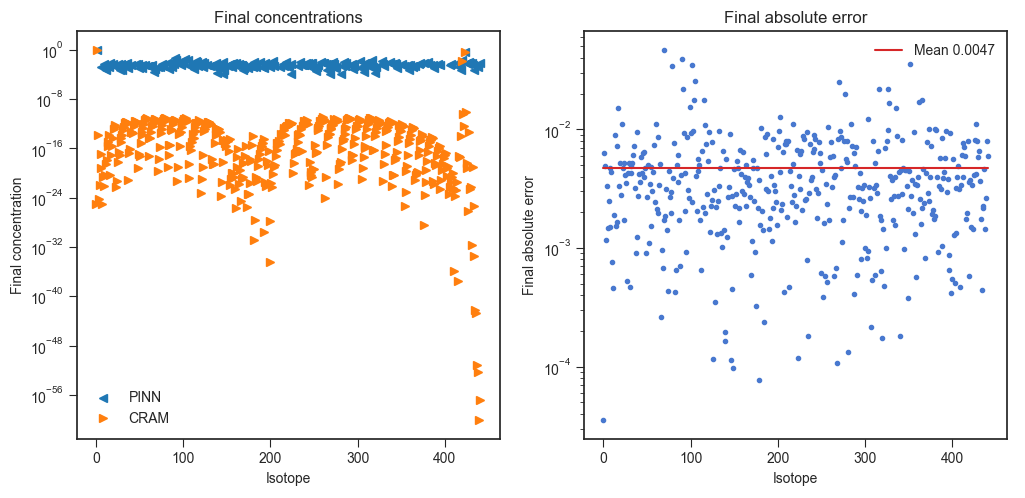
\includegraphics[width=0.85\textwidth]{burnup_over_time.png}
    % \caption{Caption}
    \label{fig:my_label}
\end{figure}
\end{frame}


\begin{frame}[fragile]{Backup slides - Weight ratio}
\begin{figure}
    \centering
    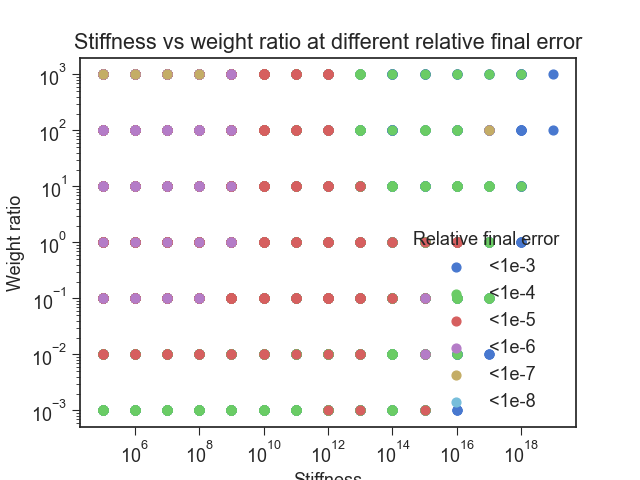
\includegraphics[width=0.85\textwidth]{stiffness_vs_weight_at_dif_error.png}
    % \caption{Caption}
    \label{fig:my_label}
\end{figure}
\end{frame}

\end{document}